\subsection*{Punto 02}

\textbf{Para cada procedimiento y para cada k, visualice la imagen comprimida usando la mejor corrida aleatoria. Cual es el menor valor de k para el cual está satisfecho con el resultado obtenido?}

Se selecciono el modelo que obtuviera la menor función objetivo dado el modelo y una k. En la figura se muestran las compresiones realizadas por cada modelo.

\begin{figure}[H]
    \centering
    \begin{subfigure}{17cm}
        \centering
        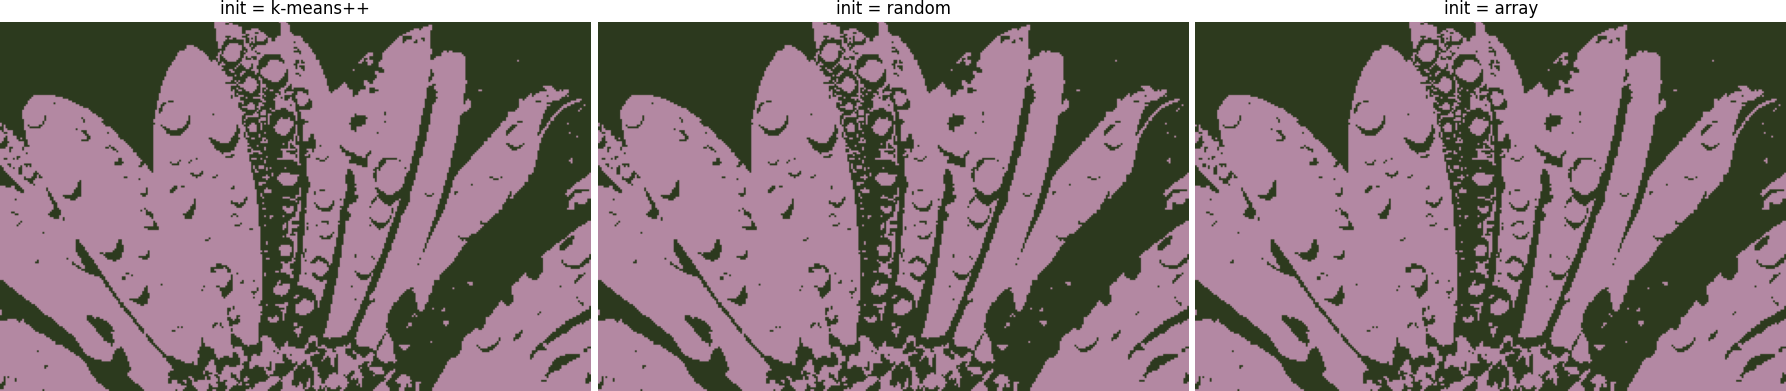
\includegraphics[width=17cm]{Graphics/Problema_04/cluster_2.png}
        \caption{K=2}
    \end{subfigure}
    \begin{subfigure}{17cm}
        \centering
        
\includegraphics[width=17cm]{Graphics/Problema_04/cluster_4.png}
        \caption{K=4}
    \end{subfigure}
    \begin{subfigure}{17cm}
        \centering
        
\includegraphics[width=17cm]{Graphics/Problema_04/cluster_8.png}
        \caption{K=8}
    \end{subfigure}
    \begin{subfigure}{17cm}
        \centering
        
\includegraphics[width=17cm]{Graphics/Problema_04/cluster_16.png}
        \caption{K=16}
    \end{subfigure}
    \begin{subfigure}{17cm}
        \centering
        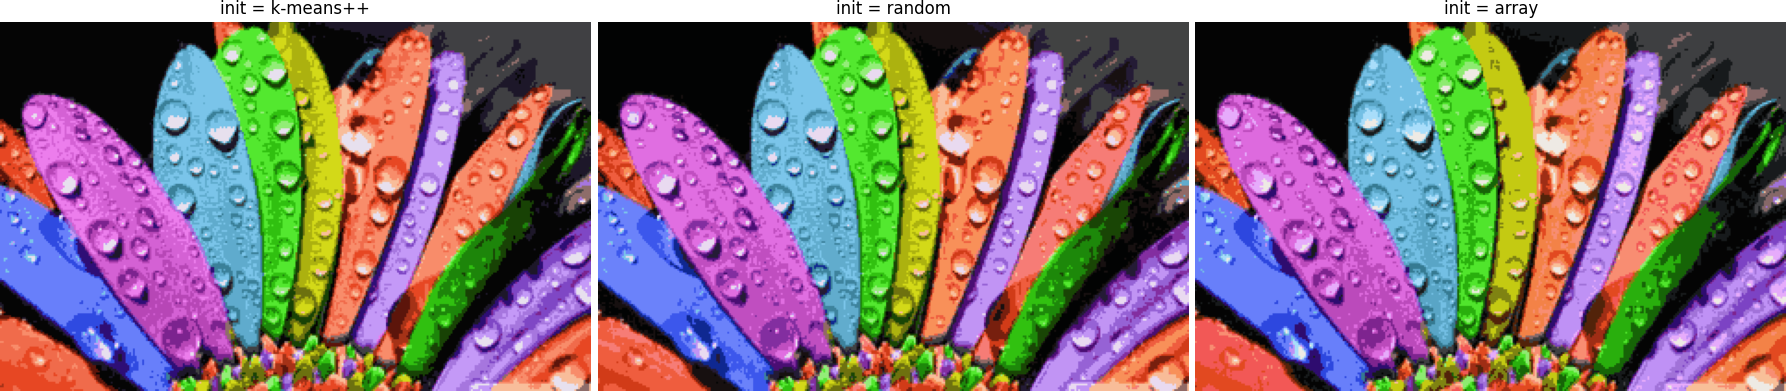
\includegraphics[width=17cm]{Graphics/Problema_04/cluster_32.png}
        \caption{K=32}
    \end{subfigure}
    \caption{Compresiones de imagenes para cada modelo y número de clusters dado.}
\end{figure}